%%%%%%%%%%%%%%%%%%%%%%%%%%%%%%%%%%%%%%%%%
% Beamer Presentation
% LaTeX Template
% Version 1.0 (10/11/12)
%
% This template has been downloaded from:
% http://www.LaTeXTemplates.com
%
% License:
% CC BY-NC-SA 3.0 (http://creativecommons.org/licenses/by-nc-sa/3.0/)
%
%%%%%%%%%%%%%%%%%%%%%%%%%%%%%%%%%%%%%%%%%

%----------------------------------------------------------------------------------------
%	PACKAGES AND THEMES
%----------------------------------------------------------------------------------------

\documentclass{beamer}

\mode<presentation> {

% The Beamer class comes with a number of default slide themes
% which change the colors and layouts of slides. Below this is a list
% of all the themes, uncomment each in turn to see what they look like.

%\usetheme{default}
%\usetheme{AnnArbor}
%\usetheme{Antibes}
%\usetheme{Bergen}
%\usetheme{Berkeley} %with Outline
%\usetheme{Berlin}
%\usetheme{Boadilla}
\usetheme{CambridgeUS} %This is well-looking
%\usetheme{Copenhagen}
%\usetheme{Darmstadt}
%\usetheme{Dresden}
%\usetheme{Frankfurt}
%\usetheme{Goettingen}
%\usetheme{Hannover}
%\usetheme{Ilmenau}
%\usetheme{JuanLesPins}
%\usetheme{Luebeck}
%\usetheme{Madrid}
%\usetheme{Malmoe}
%\usetheme{Marburg}
%\usetheme{Montpellier}
%\usetheme{PaloAlto}
%\usetheme{Pittsburgh}
%\usetheme{Rochester}
%\usetheme{Singapore}
%\usetheme{Szeged}
%\usetheme{Warsaw}

% As well as themes, the Beamer class has a number of color themes
% for any slide theme. Uncomment each of these in turn to see how it
% changes the colors of your current slide theme.

%\usecolortheme{albatross}
%\usecolortheme{beaver}
%\usecolortheme{beetle}
%\usecolortheme{crane}
\usecolortheme{dolphin}
%\usecolortheme{dove}
%\usecolortheme{fly}
%\usecolortheme{lily}
%\usecolortheme{orchid}
%\usecolortheme{rose}
%\usecolortheme{seagull}
%\usecolortheme{seahorse}
%\usecolortheme{whale}
%\usecolortheme{wolverine}

%\setbeamertemplate{footline} % To remove the footer line in all slides uncomment this line
%\setbeamertemplate{footline}[page number] % To replace the footer line in all slides with a simple slide count uncomment this line

%\setbeamertemplate{navigation symbols}{} % To remove the navigation symbols from the bottom of all slides uncomment this line
}

\usepackage{graphicx} % Allows including images
\usepackage{booktabs} % Allows the use of \toprule, \midrule and \bottomrule in tables
\usepackage{amsmath, amssymb, amsfonts}
\usepackage{mathrsfs}
\usepackage{amsthm}
%----------------------------------------------------------------------------------------
%	TITLE PAGE
%----------------------------------------------------------------------------------------

\title[VE216]{VE216 Recitation Class 8} % The short title appears at the bottom of every slide, the full title is only on the title page

\author{ZHU Yilun} % Your name
\institute[SJTU] % Your institution as it will appear on the bottom of every slide, may be shorthand to save space
{
UM-SJTU Joint Institute \\ % Your institution for the title page
\medskip
\textit{VE216 SU20 TA Group} % Your email address
}
\date{2020 Summer} % Date, can be changed to a custom date e.g.:\today

\begin{document}

\begin{frame}
\titlepage % Print the title page as the first slide
\end{frame}

\begin{frame}
\frametitle{Overview} % Table of contents slide, comment this block out to remove it
\tableofcontents % Throughout your presentation, if you choose to use \section{} and \subsection{} commands, these will automatically be printed on this slide as an overview of your presentation
\end{frame}

%----------------------------------------------------------------------------------------
%	PRESENTATION SLIDES
%----------------------------------------------------------------------------------------


%------------------------------------------------------
\section{Chapter 7: Sampling}
%------------------------------------------------------

\subsection{Sampling Theorem}
\begin{frame}
\frametitle{Sampling Theorem}
\begin{figure}
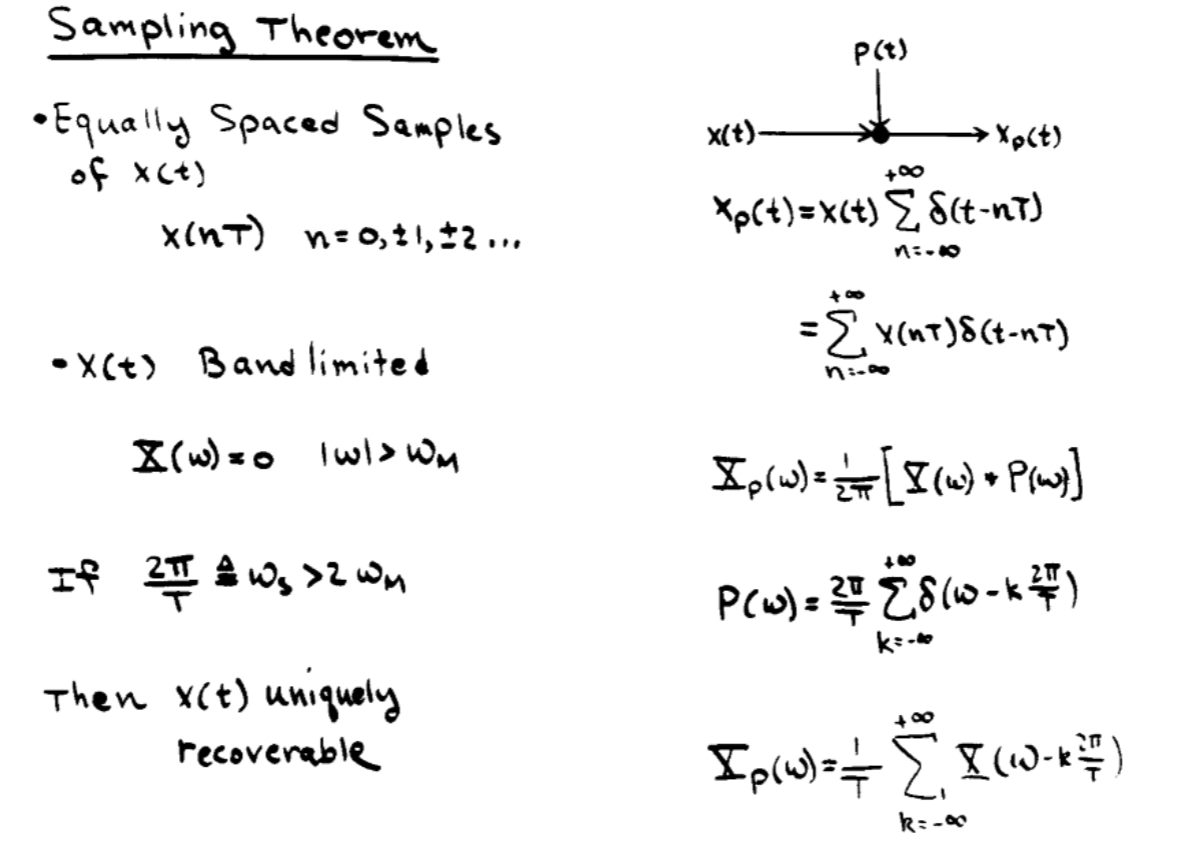
\includegraphics[width=0.8\linewidth]{sample1}
\end{figure}
\end{frame}

\begin{frame}
\frametitle{Recoverable}
\begin{figure}
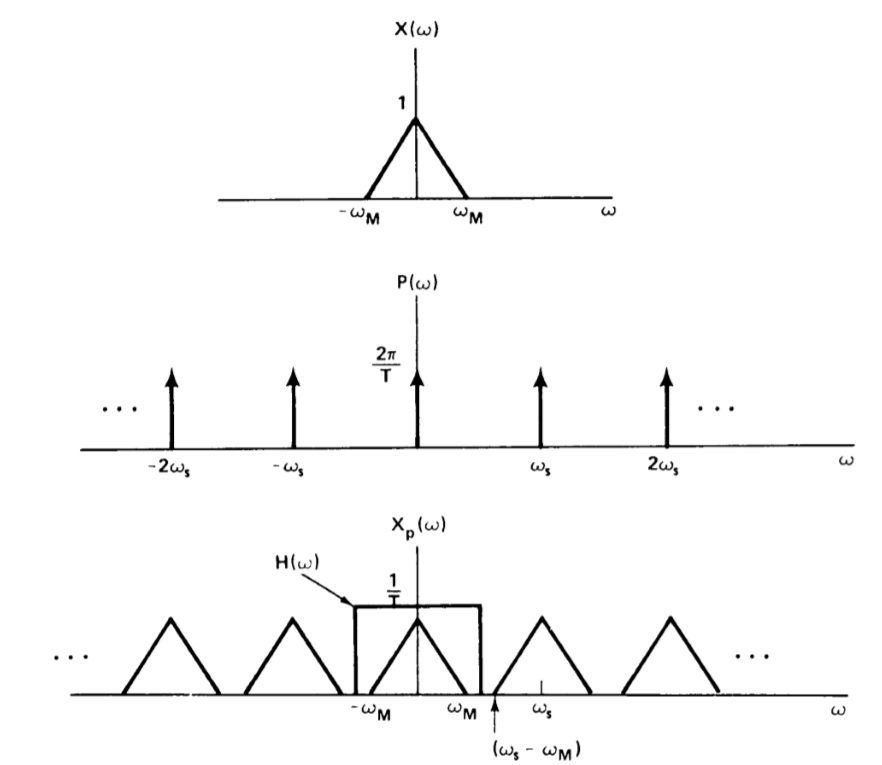
\includegraphics[width=0.7\linewidth]{sample2}
\end{figure}
\end{frame}

\begin{frame}
\frametitle{Aliasing}
\begin{figure}
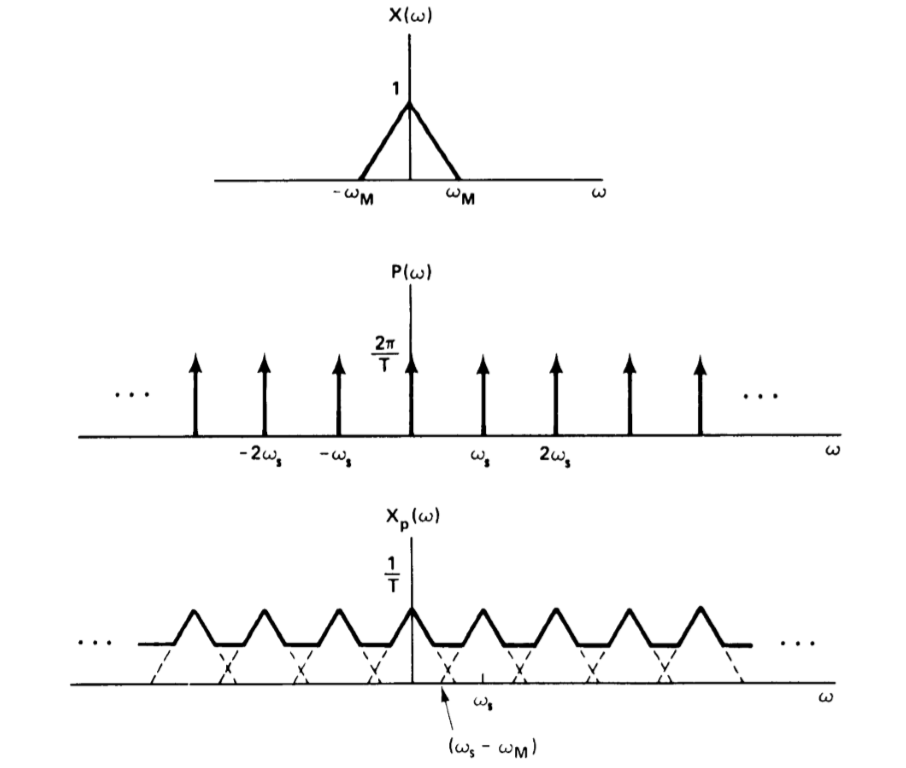
\includegraphics[width=0.7\linewidth]{sample3}
\end{figure}
\end{frame}

\subsection{Detailed Explanation of Quiz}

\begin{frame}[t]
    \frametitle{Exercise - Quiz 4 Q2}
    \begin{figure}
        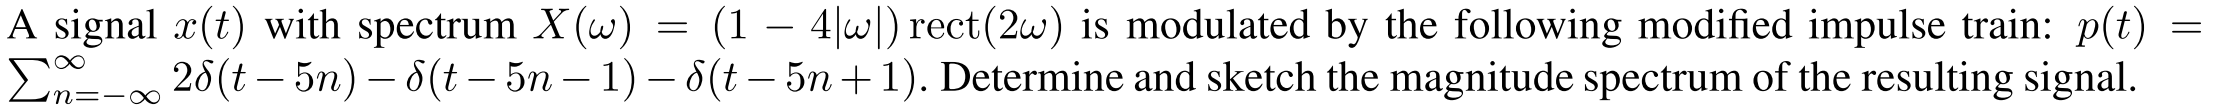
\includegraphics[width=1\linewidth]{quiz4_2.PNG}
    \end{figure}
\end{frame}

\begin{frame}[t]
    \frametitle{Exercise - Quiz 6}
    \begin{figure}
        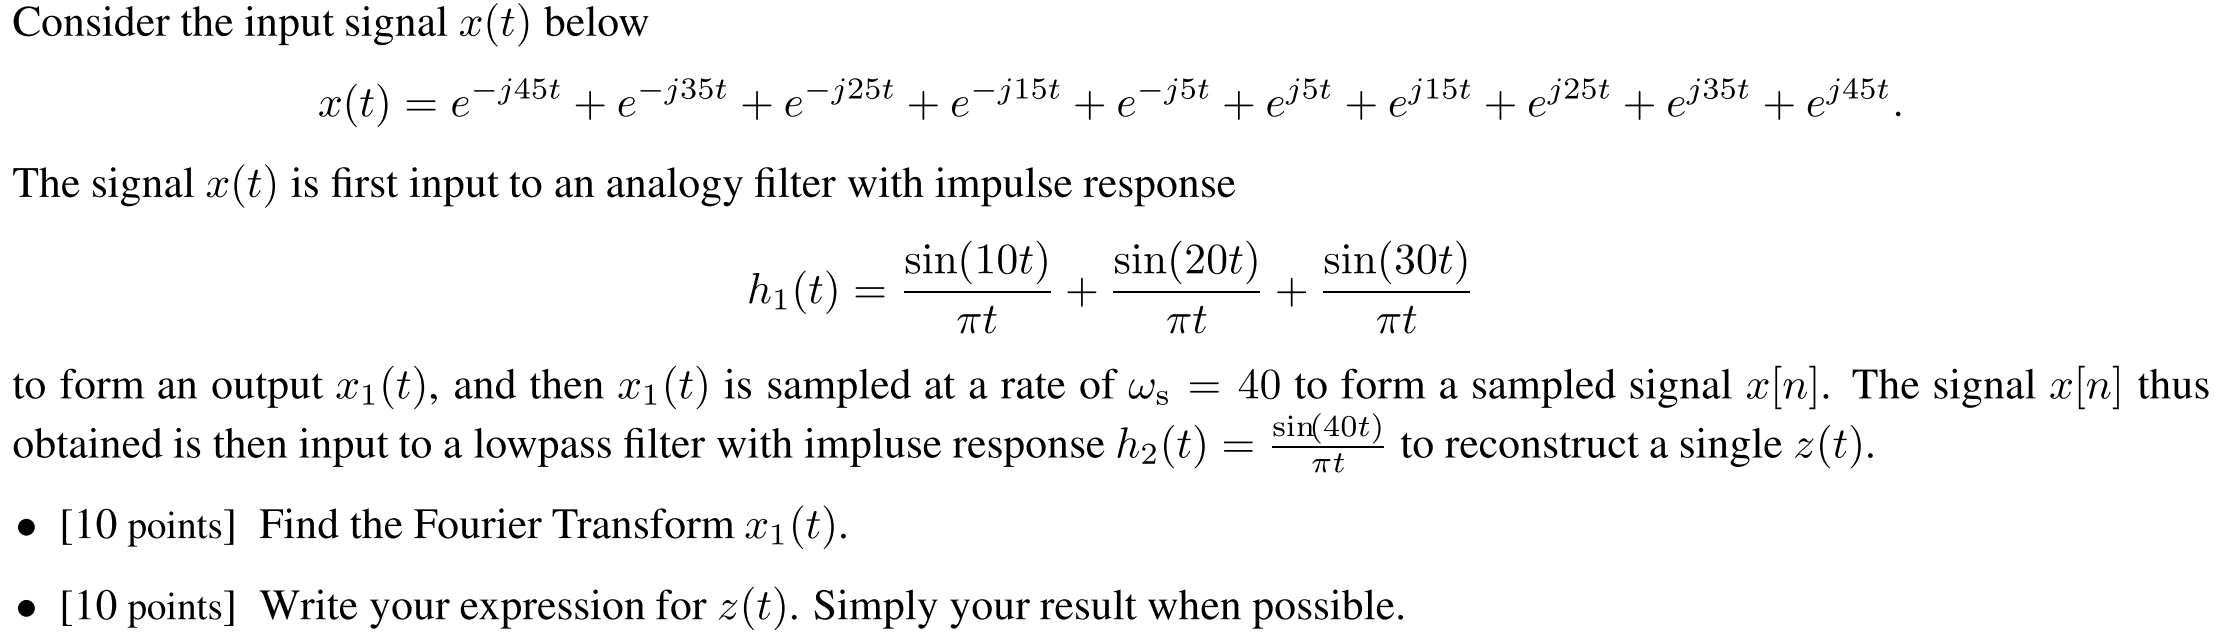
\includegraphics[width=1\linewidth]{quiz6.PNG}
    \end{figure}
\end{frame}

\begin{frame}
\frametitle{Sampling $\&$ Reconstruction}
\begin{figure}
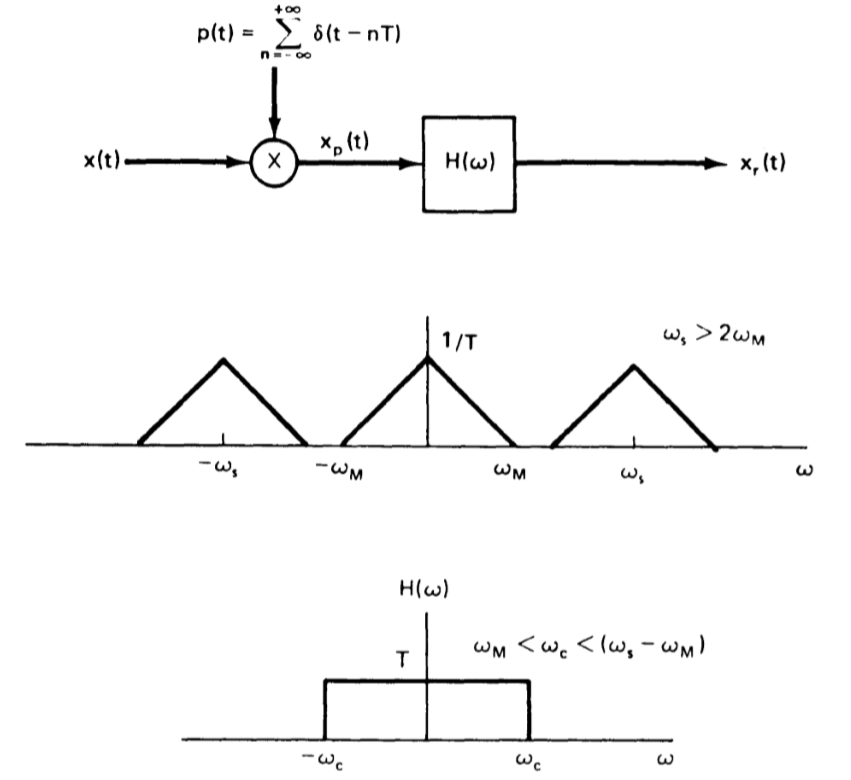
\includegraphics[width=0.6\linewidth]{sample4}
\end{figure}
\end{frame}

\begin{frame}[t]
    \frametitle{Exercise - HW5 Q6}
    \begin{figure}
        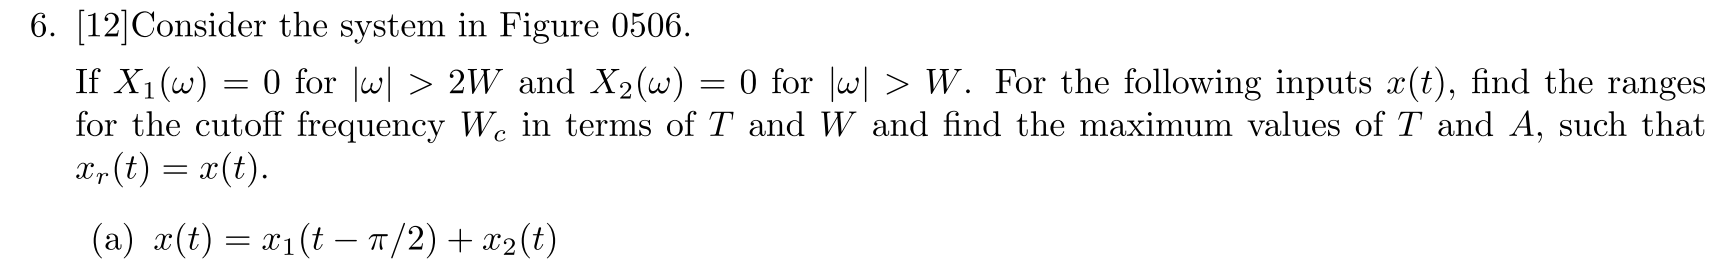
\includegraphics[width=1\linewidth]{q6a}
    \end{figure}
    \begin{figure}
        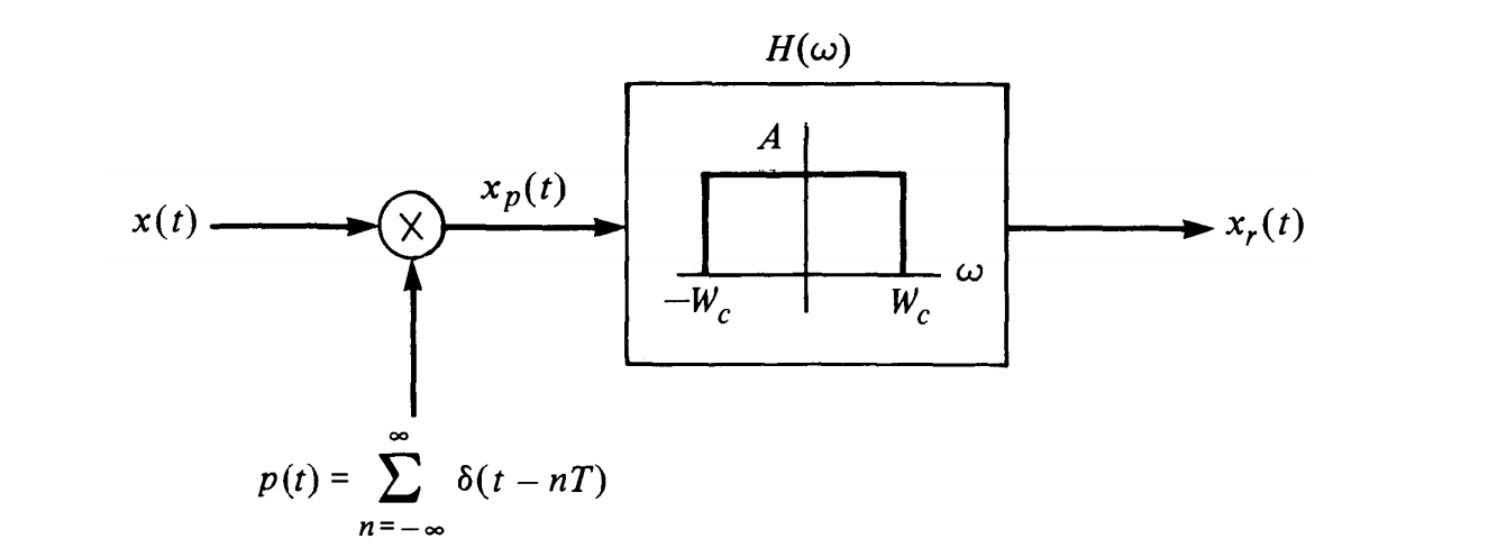
\includegraphics[width=0.6\linewidth]{q6b}
    \end{figure}
\end{frame}


\subsection{Reconstruction via Interpolation}
\begin{frame}
\frametitle{Sinc interplation (Ideal lowpass filter)}
\begin{figure}
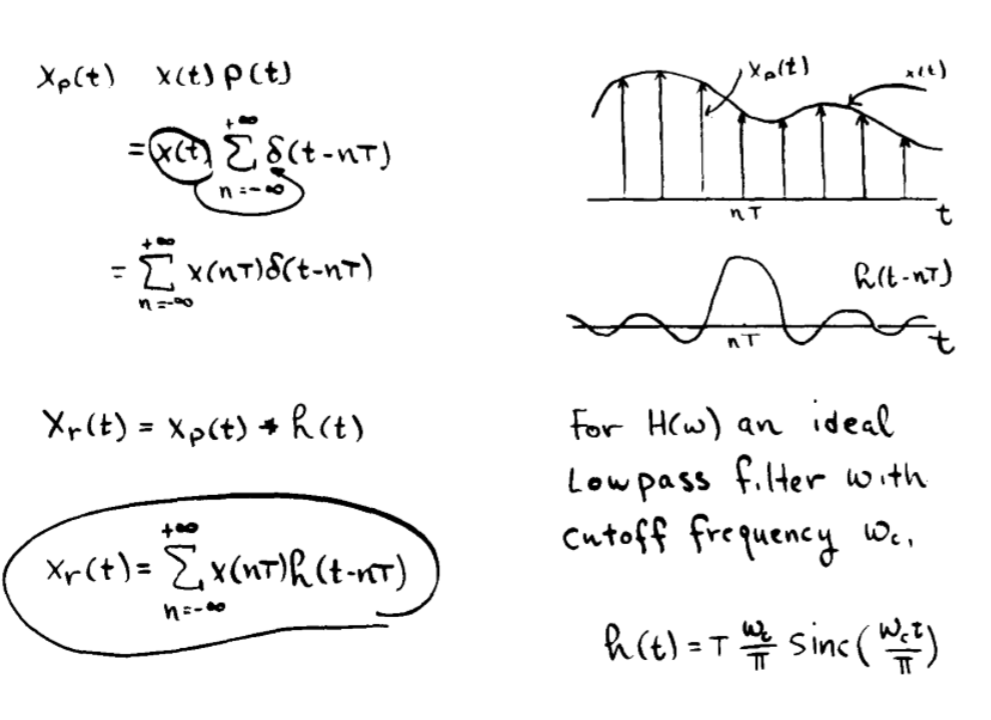
\includegraphics[width=0.7\linewidth]{sample5}
\end{figure}
\end{frame}

\begin{frame}
\frametitle{Nearest neighbor interplation (zero-order hold filter)}
\begin{figure}
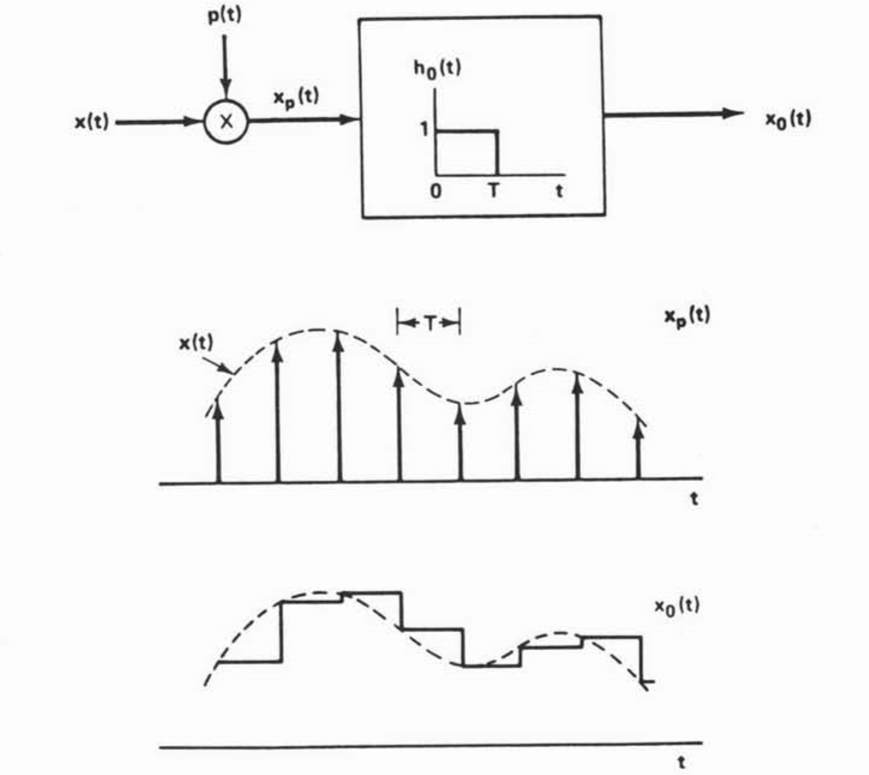
\includegraphics[width=0.7\linewidth]{sample6}
\end{figure}
\end{frame}

\begin{frame}
\frametitle{Linear interplation (first-order hold filter)}
\begin{figure}
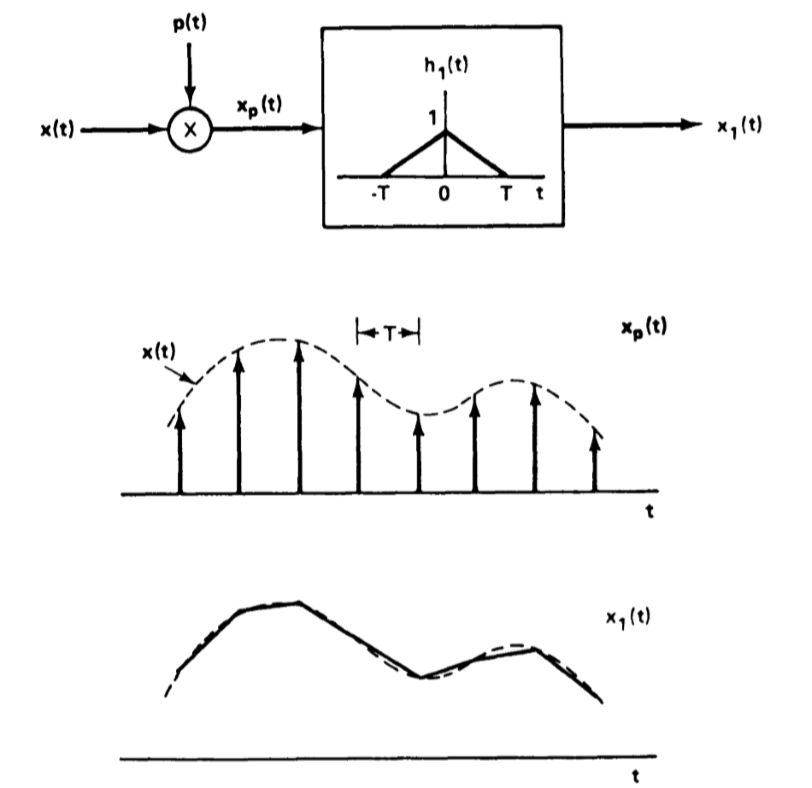
\includegraphics[width=0.7\linewidth]{sample7}
\end{figure}
\end{frame}

\begin{frame}
\frametitle{Comparison in Frequency Domain}
\begin{figure}
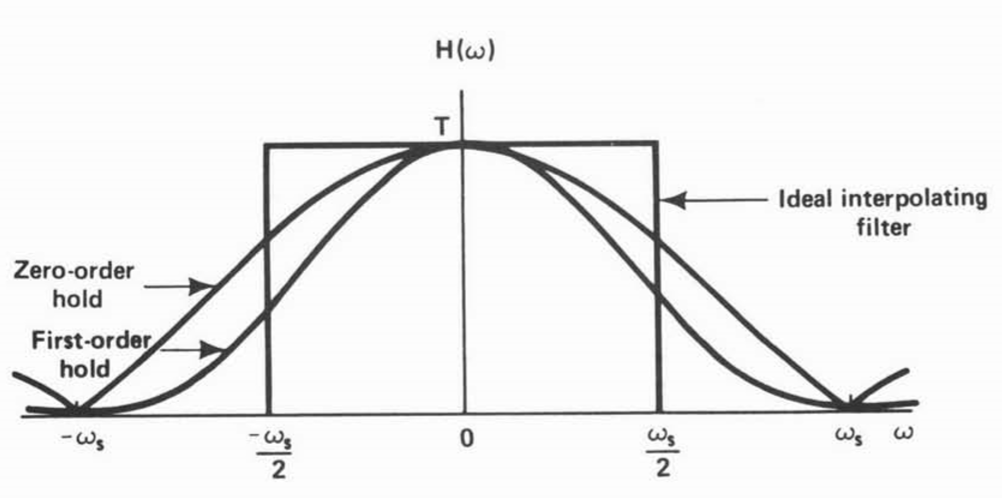
\includegraphics[width=0.7\linewidth]{sample8}
\end{figure}
\end{frame}

\begin{frame}
    \frametitle{Exercise - Interplation}
    \begin{figure}
        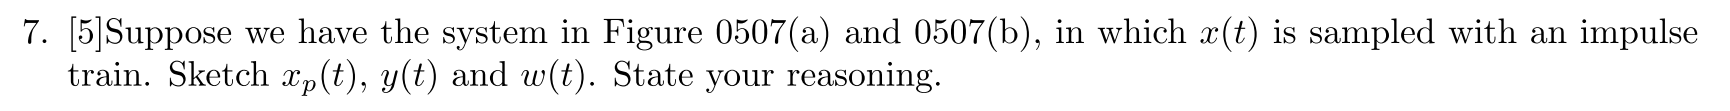
\includegraphics[width=1\linewidth]{q7a}
    \end{figure}
    \begin{figure}
        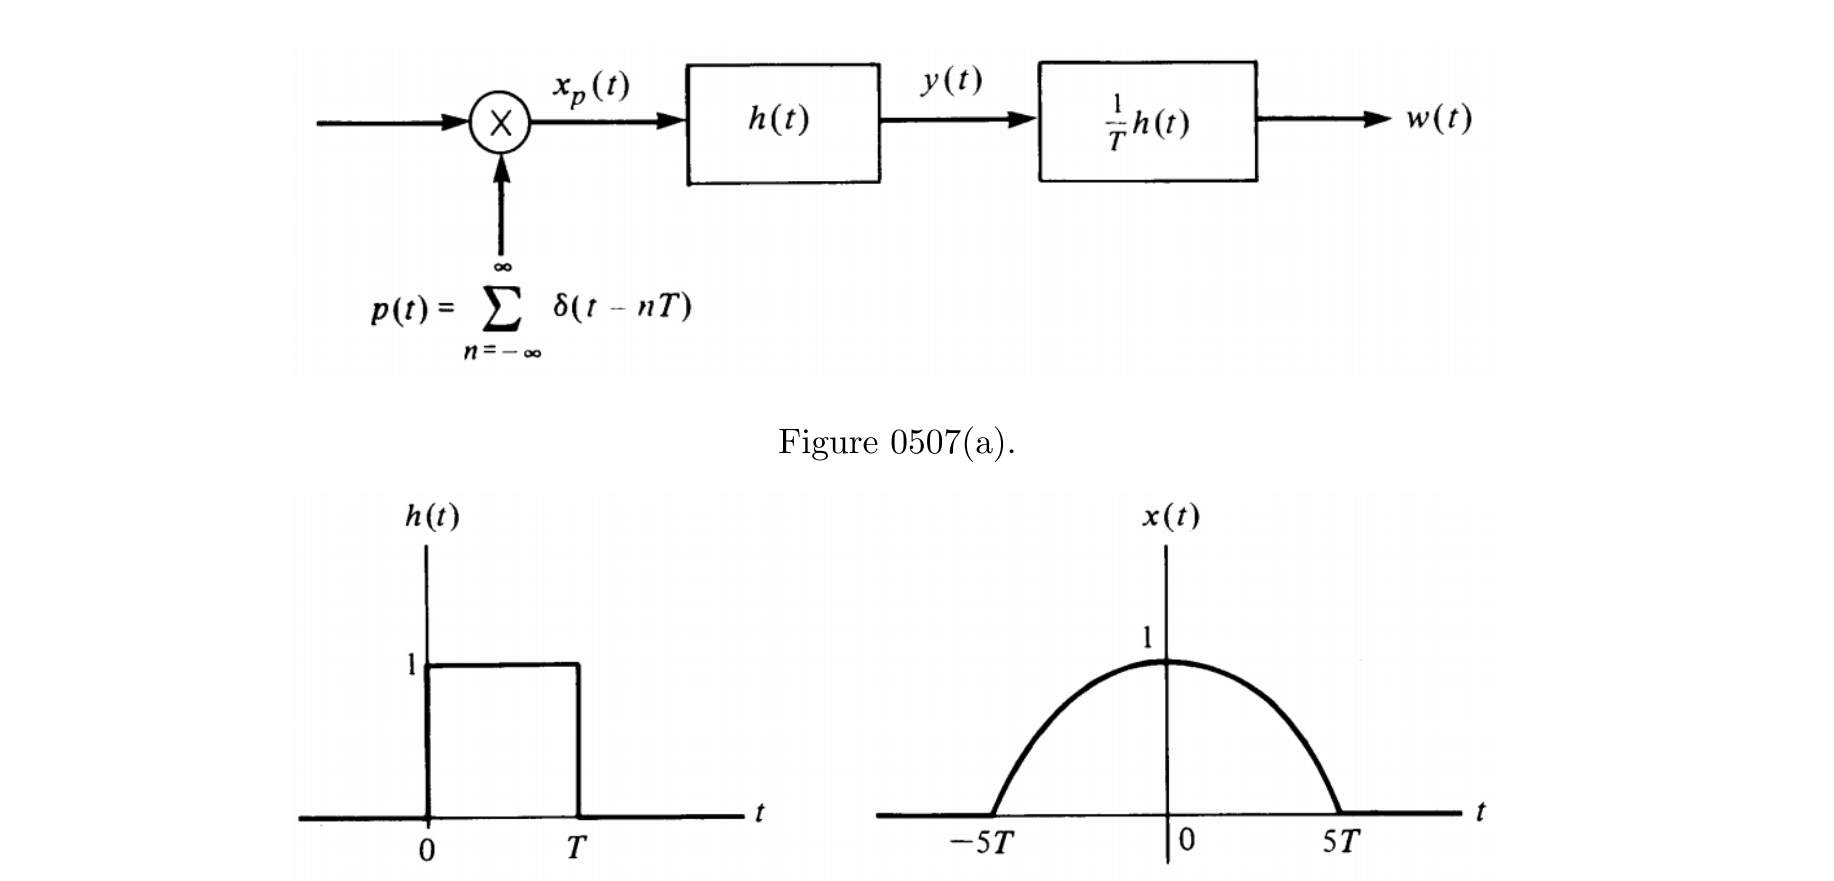
\includegraphics[width=0.8\linewidth]{q7b}
    \end{figure}

\bigskip
\bigskip
\bigskip
\bigskip
\bigskip
\end{frame}

%-------------------------------------------------
\section{Conclusion}
\begin{frame}
\frametitle{Conclusion}
\begin{itemize}
\item Time domain and Frequency behavior are consistent
\item Both sampling and reconstruction are indispensible
\item Consider eye (watching the wheels) and ear (infrasonic, ultrasonic)
\item For sampling \& reconstruction-related problems, I prefer to view them graphically (often in freq. domain).
\item Questions in HW5 are very interesting (or, tricky) - not much math involved, rather requires understanding
\end{itemize}
\end{frame}

%------------------------------------------------

\begin{frame}
\Huge{\centerline{The End}}
\end{frame}

%----------------------------------------------------------------------------------------

\end{document} 